\chapter{机器人传感技术}
\label{chap:robot-sensing}

\begin{focusbox}{本章复习路线}
看到一个传感器，先说清\textbf{测什么、如何转换、读数代表什么}。计算题优先掌握编码器的分辨角、辨向与测速，以及力和力矩的参考点变换、超声脉冲测距。简答题重点比较绝对式与增量式编码器、关节式与腕部六维力传感器，并能解释接近觉、触觉和视觉各自提供的信息。
\end{focusbox}

\section{内部状态与外部环境}

按被测对象划分，\textbf{内部传感器}提供本体状态，如关节位置、速度、加速度与内部载荷。\textbf{外部传感器}获取环境、目标或接触信息，如障碍物距离、表面压力分布与物体图像。安装在机器人上的相机仍可感知外部目标；腕部力传感器用于读出环境接触载荷时提供外部交互信息。判断分类时用被测信息和用途来说明理由。

位置反馈可采用电阻式、电容式、电感式、光电式、霍尔元件或磁栅等方法。均匀电位器在高输入阻抗读出条件下近似为分压器。若滑动端位移为 $x$、有效行程为 $l$、激励电压为 $U_e$，并以滑动起点为低电位端，则 $U_o\simeq U_e x/l$。旋转电位器可把 $x/l$ 换成角行程比例。传感器选型同时检查量程、分辨率、定位误差、重复性、动态响应和工作环境。

\section{旋转编码器}
\label{sec:rotary-encoders}

\subsection{绝对式读码与增量式计数}

\dfn{绝对式编码器}{输入轴转到某个角区时，多条码道同时给出该角区的码字。若 $n$ 位码覆盖一整圈并均匀编码，单圈位置数为 $2^n$，最小分辨角为 $\Delta\theta=360^\circ/2^n$。单圈绝对码上电可读出圈内位置，圈数需要多圈能力或其他信息。}

光学式绝对编码器通过检测各码道的透光与遮光状态读位，也可用接触型码盘帮助理解编码结构。自然二进制从 $0111$ 切到 $1000$ 时多位同时变化，边界处各码道的读出时刻若有偏差，可能产生跳码。格雷码的相邻位置只变一位，可减少这种多位跳变错误。编码读取后需按实际码制译码。对反射格雷码，从最高位向最低位用 $b_{n-1}=g_{n-1}$，$b_k=b_{k+1}\oplus g_k$ 恢复自然二进制。

\begin{figure}[htbp]
\centering
\begin{minipage}[b]{.542\linewidth}
\centering
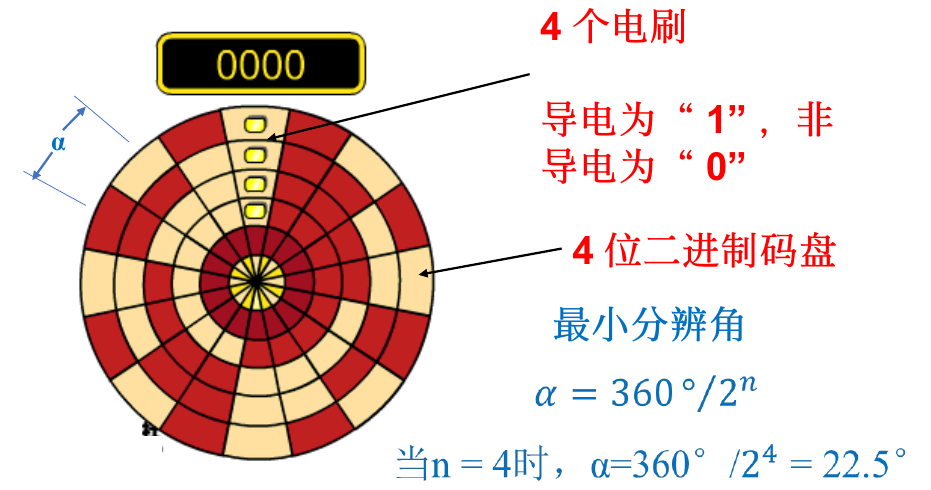
\includegraphics[width=\linewidth]{02-absolute-code-disc.png}\\[-.1em]
{\small (a) 接触式四位绝对码盘}
\end{minipage}\hfill
\begin{minipage}[b]{.425\linewidth}
\centering
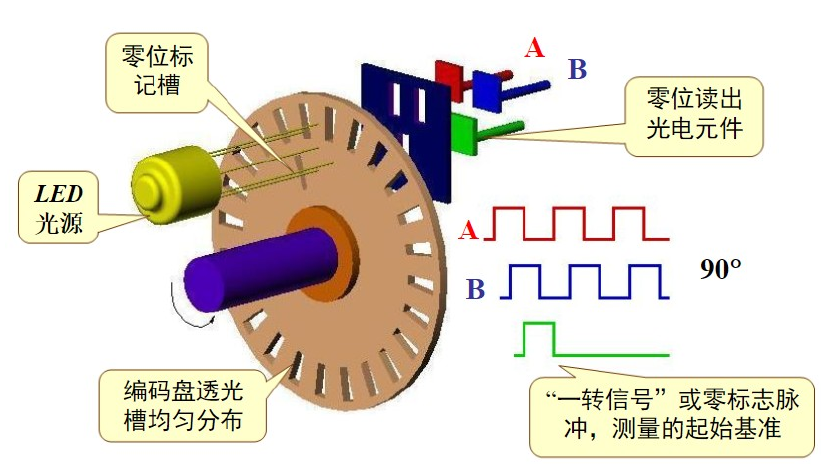
\includegraphics[width=\linewidth]{02-incremental-encoder.png}\\[-.1em]
{\small (b) 增量式光电编码器}
\end{minipage}
\caption{绝对式码盘的多码道与增量式编码器的 A/B/Z 信号。取自《第2章：机器人传感技术》第12、15张。}
\label{fig:encoder-principle}
\end{figure}

增量式编码器的透光条纹产生周期脉冲。A、B 相相差 $90^\circ$ 电相位，讲义约定 A 超前 B 时为正转，反过来为反转。该相位差是单个信号周期的四分之一。Z 相通常每转一脉冲，可在回零流程中提供参考标志。正交解码可数 A 相单边沿（$m=1$）、A 相双边沿（$m=2$）或 A、B 相全部边沿（$m=4$）。约定 $P$ 为 A 相每转的完整周期数，在同一解码方式下
\[
C=mP,\qquad \Delta\theta=\frac{2\pi}{C},\qquad
\theta-\theta_{\mathrm{ref}}=n_c\frac{2\pi}{C},\qquad
\overline\omega=\frac{2\pi\Delta n_c}{C\Delta t}.
\]
其中 $C$ 为实际每转计数，$n_c$ 是自参考位置累加的带符号计数。若手册已直接给出每转计数，应以该计数为 $C$。停电后若累加计数丢失，需重建参考位置。用固定时间窗测速时，低速可能只读到少数计数，可采用边沿间隔估计或在允许延迟时加长时间窗。

\nt{\textbf{分辨率、精度与安装位置}　解码倍频缩小名义分辨角。称为角度精度时还要考虑码盘偏心、相位误差和机械间隙。电机侧编码器经减速比换算得到理想关节读数；关节输出端的间隙、弹性变形需另行建模或测量。}

\ex{增量式编码器的转角和转速}{电机编码器 A 相每转 $1024$ 个完整周期，A、B 相所有边沿均计数。$40\,\mathrm{ms}$ 内计数净增 $128$，采用 A 超前 B 为正向的约定。求电机角增量与平均转速。若电机经同向理想 $8{:}1$ 减速器带动关节，再求关节侧数值。}

\textbf{解}　四倍计数时 $C=4096$，所以电机轴一计数对应 $360^\circ/4096=0.08789^\circ$。窗口内角增量及平均转速为
\[
\Delta\theta_m=\frac{128}{4096}\,360^\circ=11.25^\circ,
\qquad n_m=\frac{128}{4096\times0.040}\,60=46.875\,\mathrm{rpm}.
\]
关节角增量为 $1.40625^\circ$，平均转速为 $5.859375\,\mathrm{rpm}$。角增量和速度都带正号。若换用 A 相单边沿计数，同一实际转角只产生 $32$ 个计数，重新用 $C=1024$ 换算也得到同样的角增量。

\ex{绝对式编码器的格雷码译码}{四位单圈绝对式编码器采用反射格雷码，当前输出 $1000$，设自然二进制零码对应 $0^\circ$，正向每级角度按均匀格点换算。求角度标称值。}

\textbf{解}　逐位异或有 $b_3=1$、$b_2=1\oplus0=1$、$b_1=b_0=1$，得到自然二进制 $1111=15$。每级分辨角 $360^\circ/16=22.5^\circ$，标称位置为 $15\times22.5^\circ=337.5^\circ$。原码 $1000$ 与下一圈零码 $0000$ 也只相差一位。

\FloatBarrier
\section{力、力矩与六维力传感}
\label{sec:robot-force-sensing}

\subsection{机械载荷如何变为电信号}

关节式力矩传感器通常测单个关节轴的转矩。载荷使弹性元件发生扭转，应变片把应变变为相对电阻变化 $\Delta R/R=K_g\varepsilon$，再经激励电桥读出电压。测量链可写成
\[
\text{关节转矩}\longrightarrow\text{弹性变形}\longrightarrow
\varepsilon\longrightarrow\Delta R\longrightarrow U_o .
\]
在线性区，若等臂单臂电桥的受拉应变片是输出支路的下臂，输出取该支路中点电压减参考支路中点电压，则 $U_o\simeq U_e K_g\varepsilon/4$。接法决定输出极性，实际标定把电压映射回转矩。

腕部六维力传感器通常安装在机械臂腕部与末端工具之间，提供三个力分量和关于指定参考点的三个力矩分量。选择不同弹性结构与应变片位置，使各加载方向产生可区分的应变组合。若若干通道的读数为 $\mathbf y$，定义力旋量 $\boldsymbol w=[F_x,F_y,F_z,M_x,M_y,M_z]^{\mathsf T}$。线性标定可写为
\[
\mathbf y=\mathbf A\boldsymbol w+\mathbf b .
\]
$\mathbf b$ 为零点偏置。方阵 $\mathbf A$ 可逆时，用 $\mathbf A^{-1}(\mathbf y-\mathbf b)$ 恢复六个分量；对多通道满列秩的情形可用最小二乘标定与解算。标定矩阵的非对角耦合反映单通道可能同时响应多个力或力矩分量。

\begin{figure}[htbp]
\centering
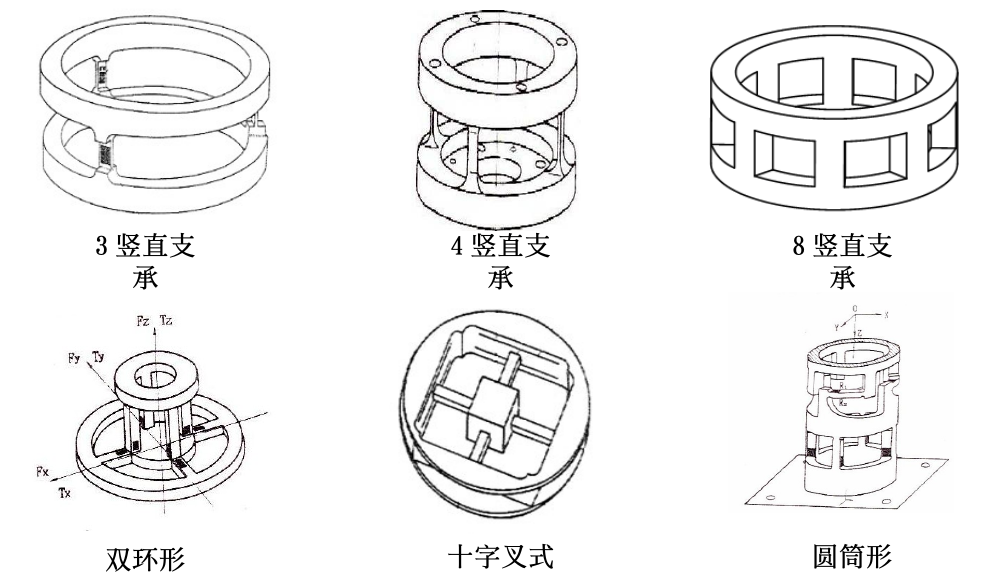
\includegraphics[width=.73\linewidth]{02-six-axis-structures.png}
\caption{腕部六维力传感器的几种弹性体结构。取自《第2章：机器人传感技术》第20张。}
\label{fig:six-axis-structures}
\end{figure}

\subsection{力矩的参考点与无传感器估计}

同一个力用同一坐标轴表示时，改变参考点只改变对应力矩。若 $\boldsymbol r_{OC}$ 从新参考点 $O$ 指向原参考点 $C$，则
\[
\boldsymbol F_O=\boldsymbol F_C,\qquad
\boldsymbol M_O=\boldsymbol M_C+\boldsymbol r_{OC}\times\boldsymbol F_C .
\]
若坐标轴同时改变，还应把两个三维向量旋转到同一坐标系后再做叉乘。

也可由电机电流 $\tau_e=K_t i_a$ 估计电磁转矩，经传动折算并扣除机器人惯性、重力、摩擦等模型项后，估计外力在关节上的等效转矩。以 $\boldsymbol w_{\mathrm{ext}}$ 表示环境作用于机器人、与雅可比 $\mathbf J$ 用同一坐标系、参考点和力/速度分量顺序表示的力旋量。由虚功关系
\[
\boldsymbol\tau_{\mathrm{ext}}^{\mathsf T}\delta\boldsymbol q
=\boldsymbol w_{\mathrm{ext}}^{\mathsf T}\mathbf J\delta\boldsymbol q
\quad\Longrightarrow\quad
\boldsymbol\tau_{\mathrm{ext}}=\mathbf J^{\mathsf T}\boldsymbol w_{\mathrm{ext}} .
\]
单末端接触假设下，能否由关节残差唯一估计六维力旋量取决于 $\mathbf J$ 的秩。摩擦误差、模型误差、未知接触位置与奇异位形都会影响估计。

\Needspace{12\baselineskip}
\ex{腕部测力中的参考点}{传感器与接触点的坐标轴平行。从腕部传感器原点 $O$ 指向接触点 $C$ 的位置向量为 $(0.06,0.02,0)^{\mathsf T}\,\mathrm m$。接触点有力 $\boldsymbol F_C=(0,0,20)^{\mathsf T}\,\mathrm N$ 和力矩 $\boldsymbol M_C=(0,0,0.10)^{\mathsf T}\,\mathrm{N\,m}$。求关于 $O$ 的六维载荷。}

\textbf{解}　力分量保持原值，力作用点平移造成附加力矩
\[
\boldsymbol r_{OC}\times\boldsymbol F_C
=\begin{bmatrix}0.02\times20\\-0.06\times20\\0\end{bmatrix}
=\begin{bmatrix}0.40\\-1.20\\0\end{bmatrix}\,\mathrm{N\,m}.
\]
故关于腕部原点的力矩为 $(0.40,-1.20,0.10)^{\mathsf T}\,\mathrm{N\,m}$，与力 $(0,0,20)^{\mathsf T}\,\mathrm N$ 组成六维载荷。若已知腕部读数并要换算到接触点，则减去上述附加力矩。

\FloatBarrier
\section{接近觉、测距与触觉}

\begin{table}[htbp]
\centering\small
\begin{tabularx}{\linewidth}{@{}p{2.2cm} X X@{}}
\toprule
方式 & 转换链 & 使用条件 \\
\midrule
电涡流 & 线圈交变磁场在导电目标中激起涡流，涡流反作用改变线圈阻抗。 & 适合导电目标的近距离检测，读数也随材料与几何条件变化。 \\
超声波 & 发射脉冲，接收回波；已知声速 $c$ 和往返时差 $\Delta t$，得 $d=c\Delta t/2$。 & 声速随介质和温度变化；发射振铃造成近场盲区，倾斜或吸声面可能回波弱。 \\
主动红外 & 发射调制红外光，接收目标反射后解调，可判断物体接近。 & 与目标表面反射率、入射角及背景光有关。反射强度式需标定，测距型还可用三角或飞行时间原理。 \\
\bottomrule
\end{tabularx}
\end{table}

\textbf{触觉信息有层次。}开关式触觉只提供接触与否；分布式接触传感器还能定位接触区域；压觉或力觉给出接触强弱；滑觉用来识别物体与夹爪的相对滑动，便于调节握持力。压阻阵列的行、列电极交叉处构成触元，受压使局部电阻改变，逐行列扫描可恢复压力分布。性能受触元密度、灵敏度、柔顺性和耐用性共同约束。探测到压强 $p_k$ 的触元有效面积为 $A_k$ 时，各触元法向力近似为 $p_kA_k$；在接触面近似平坦且压力方向平行时可由 $\sum_k p_kA_k$ 估算法向总力。

\begin{figure}[htbp]
\centering
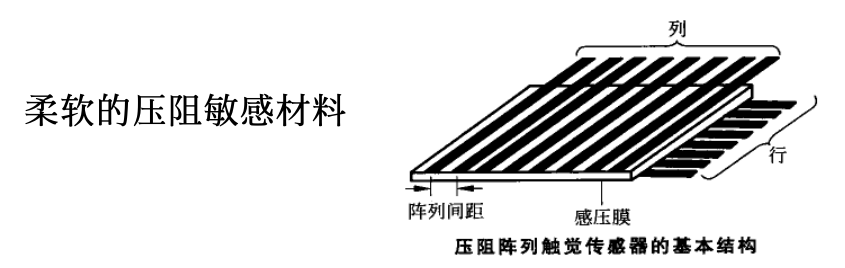
\includegraphics[width=.71\linewidth]{02-tactile-array.png}
\caption{压阻阵列的行列电极与触元结构。取自《第2章：机器人传感技术》第30张。}
\label{fig:tactile-array}
\end{figure}

\ex{超声飞行时间测距}{一只同处发射与接收的超声测距模块，在已知空气声速 $c=343\,\mathrm{m/s}$ 的条件下测得脉冲往返时间为 $8.0\,\mathrm{ms}$。忽略内部延迟，求单程障碍物距离。}

\textbf{解}　$\Delta t$ 覆盖从传感器到障碍物再返回的路程，故 $d=343\times0.0080/2\approx1.37\,\mathrm m$。若电路有固定延迟，先从实测时差中扣除该延迟再代入飞行时间公式。

\FloatBarrier
\Needspace{8\baselineskip}
\section{视觉传感器与成像元件}

视觉系统通常由照明、镜头、相机、图像处理器和算法组成。先用照明把目标特征和背景分开，再由镜头成像，传感器完成光电转换和场景离散化，图像算法提取控制需要的目标信息。检测轮廓时可考虑背光突出边界，观察表面细节时则可用适合反射特性的照明。

\begin{itemize}
\item \textbf{焦距与视场}　在传感器尺寸和成像模型固定时，较短焦距给出较大视场角。理想直线投影的水平视场角可近似为 $2\arctan(w/(2f))$，其中 $w$ 为有效传感器宽度，$f$ 为焦距。镜头分类应结合画幅和投影方式，鱼眼镜头的投影关系要单独考虑。
\item \textbf{光圈与景深}　光圈数 $N_f=f/D$，$D$ 为入瞳直径。光圈数增大时开口相对缩小；在相同焦距、对焦距离和弥散标准下，通常进光减少而景深增大。缩得过小时，衍射也会影响清晰度。
\item \textbf{CCD 与 CMOS}　两者都利用光生电荷感光。典型 CCD 逐级转移电荷，汇至少数输出节点转换并读出；典型 CMOS 在像素有电荷电压转换能力，可借助行列寻址与并行通道读出，便于实现高集成和低功耗。噪声、帧率及动态范围需按器件规格与曝光方式判断。
\end{itemize}

\begin{focusbox}{考前自测}
\begin{enumerate}
\item 已知 $12$ 位单圈绝对编码器和 $1024$ 周期/转的增量式编码器（四倍计数），二者名义分辨角有何关系？各自的读数如何对应角位置？
\item 只测腕部法向力大小时，能否区分同方向等大小但作用点不同的两个力？六维传感器多提供了什么信息？
\item 对金属近接检测、移动机器人障碍物测距、夹持滑动判断，各选哪类传感器？
\end{enumerate}
\textbf{核对}　两者均为 $360^\circ/4096$；绝对式直接译码得到圈内位置，增量式由参考点和带符号计数求位置。法向力一样时需利用关于同一参考点的力矩分量判断力线偏移。三项任务分别可用电涡流探头、超声脉冲测距模块与滑觉传感器。
\end{focusbox}

{\small 本章依据《第2章：机器人传感技术》第3至4、7至15、17至30、33至41张整理。格雷码、四倍计数、分辨率与精度的辨析也参考《编码器核心技术深度解析与应用趋势》第7、9、13页。}
